

\documentclass[a4paper, norsk, 12pt]{article}
\usepackage[utf8]{inputenc}
\usepackage[T1]{fontenc}
\usepackage{babel, textcomp, color, amsmath, amssymb, tikz, subfig, float,esint}
\usepackage{amsfonts}
\usepackage{graphicx}

\usepackage{tikz}
\usepackage{pgfplots}
\usepackage{collectbox}

\usepackage{mathtools}
\usepackage{empheq}
\usepackage[skins,theorems]{tcolorbox}
\tcbset{highlight math style={enhanced,
  colframe=red!60!black,colback=white,arc=4pt,boxrule=1pt}}
\definecolor{myblue}{rgb}{.9529, .9333, 0.8274}
\newcommand*\mybluebox[1]{%
\colorbox{myblue}{\hspace{1em}#1\hspace{1em}}}
% USEAGE:
%		\begin{empheq}[box=\mybluebox]{align}
%		A =  \left( \frac{1}{ 2\pi a^2}\right)^{\frac{1}{4}}
%		\end{empheq}

\makeatletter

\newcommand{\BOX}[1]{
\begin{empheq}[box=\mybluebox]{align}
#1
\end{empheq}
}

\newcommand{\EQU}[1] { \begin{equation*} \begin{split}
#1  
\end{split} \end{equation*} }
 \newcommand{\DE}[1] {  \begin{description}  #1 \end{description} }
 \newcommand{\IT}[2] { \item[\color{blue} #1]{#2} }
 \newcommand{\vv}[1] { \mathbf{#1} }
 \newcommand{\PAR}[2]{ \frac{\partial #1}{\partial #2}}
 \newcommand{\ket}[1] { |#1\rangle }
 \newcommand{\expe}[1]{ \langle #1 \rangle }
  \newcommand{\bra}[1] { \langle #1 | }
  \newcommand{\braket}[2] { \langle #1 | #2 \rangle }
  \newcommand{\colvec}[2] { 
  \left( \begin{matrix}
 #1 \\
 #2 \\
  \end{matrix}\right) }
 \newcommand{\PLOTS}[4]{ 
\begin{tikzpicture}
\begin{axis}[
    axis lines = #3, %usally left
    xlabel = #1,
    ylabel = #2,
]
#4
\end{axis}
\end{tikzpicture}
}

\newcommand{\addPLOT}[4]{
\addplot [domain=#1:#2,samples=200,color=#3,]{#4};}
\newcommand{\addCOORDS}[1]{\addplot coordinates {#1};}
\newcommand{\addDRAW}[1]{\draw #1;}
\newcommand{\addNODE}[2]{ \node at (#1) {#2};}

%		\PLOTS{x}{y}{left}{
%			\ADDPLOT{x^2}{-2}{2}{blue}
%			\ADDCOORDS{(0,1)(1,1)(1,2)}
%		}




\definecolor{svar}{RGB}{0,0,0}
\definecolor{opgavetekst}{RGB}{109,109,109}
\definecolor{blygraa}{RGB}{44,52,59}


\title{ 
\Huge ---------------ENT3R--------------- \\ \large Geometriske argumenter}
\author{ August Geelmuyden og Sindre Bilden \\
\huge --------------------------------------------
}
\date{}
\begin{document}
  \maketitle

\section*{Introduksjon}
Det å ha en geometrisk forståelse av matematiske formler gjør ofte at formlene fremstår klarere. Derfor valgte vi ut en rekke matematiske formler elevene ble bedt om å forklare ved hjelp av å tegne figurer.\\[0.5cm]
Vi skrev formlene på lapper og ba elevene velge én hver. Elevene fikk sitte i et kvarter med formlene imens vi gikk rundt og ga små hint. Etterpå lot vi elevene presentere formlene på tavlen. 
 
\section*{Elevenes reaksjon}
Elevene syntes det var krevende å lage figurene, men syntes det var gøy å se matematikk på denne måten. Formlene var krevende å visualisere, opplegget krever derfor mye hjelp fra mentorene. \\

\section*{Noen formler}
\begin{itemize}
\item Første kvadratsetning: $(a+b)^2=a^2+2ab+b^2$
\item Andre kvadratsetning: $(a-b)^2=a^2-2ab+b^2$
\item Konjugatsetningen: $(a+b)(a-b)=a^2-b^2$
\item Pythagoras læresetning: $a^2=b^2+c^2$
\item Trigonometrisk identitet: $\sin^2\theta+\cos^2\theta=1$
\item Uendelig geometrisk rekke: $\frac{1}{2}+\frac{1}{4}+\frac{1}{8}+...+\frac{1}{2^n}+...=1$
\item Trappesum: $1+2+3+4+...+(N-1)+N=\frac{1}{2}N(N+1)$
\item Kryssleddulikhet: $a^2+b^2\geq 2ab$
\item Delelighet: \textit{Dersom $a$ er et positivt heltall og $a^2$ er et partall, må $a^2$ være delelig med 4. (Det vil si: $\frac{1}{4}a^2$ må være et heltall.)}
\item Oddetallssum: \textit{Summen av de $n$ første oddetallene er $n^2$.}
\end{itemize}

Under følger et utvalg av oppgaver og elevenes/våre forslag til visuell løsning. 
\subsection*{OPPGAVE: $(a+b)^2=a^2+2ab+b^2$}
\subsection*{LØSNING:}
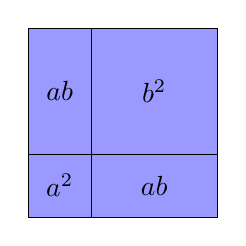
\begin{tikzpicture}[scale=0.8]
\filldraw[fill=blue!40] (0,0) -- (0,1) -- (1,1) -- (1,0) --cycle; % a^2
\draw (0.5,0.5) node{$a^2$};
\filldraw[fill=blue!40] (1,1) -- (1,3) -- (3,3) -- (3,1) --cycle; % b^2
\draw (2,2) node{$b^2$};
\filldraw[fill=blue!40] (1,0) -- (3,0) -- (3,1) -- (1,1) --cycle;
\draw (2,0.5) node{$ab$};
\filldraw[fill=blue!40] (0,1) -- (0,3) -- (1,3) -- (1,1) --cycle;
\draw (0.5,2) node{$ab$};
\end{tikzpicture}
$=$
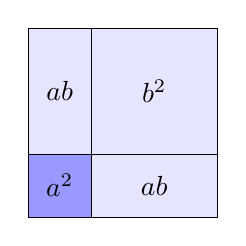
\begin{tikzpicture}[scale=0.8]
\filldraw[fill=blue!40] (0,0) -- (0,1) -- (1,1) -- (1,0) --cycle; % a^2
\draw (0.5,0.5) node{$a^2$};
\filldraw[fill=blue!10] (1,1) -- (1,3) -- (3,3) -- (3,1) --cycle; % b^2
\draw (2,2) node{$b^2$};
\filldraw[fill=blue!10] (1,0) -- (3,0) -- (3,1) -- (1,1) --cycle;
\draw (2,0.5) node{$ab$};
\filldraw[fill=blue!10] (0,1) -- (0,3) -- (1,3) -- (1,1) --cycle;
\draw (0.5,2) node{$ab$};
\end{tikzpicture}
$+$
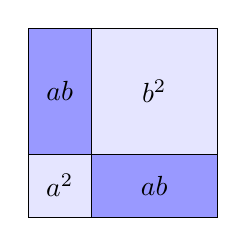
\begin{tikzpicture}[scale=0.8]
\filldraw[fill=blue!10] (0,0) -- (0,1) -- (1,1) -- (1,0) --cycle; % a^2
\draw (0.5,0.5) node{$a^2$};
\filldraw[fill=blue!10] (1,1) -- (1,3) -- (3,3) -- (3,1) --cycle; % b^2
\draw (2,2) node{$b^2$};
\filldraw[fill=blue!40] (1,0) -- (3,0) -- (3,1) -- (1,1) --cycle;
\draw (2,0.5) node{$ab$};
\filldraw[fill=blue!40] (0,1) -- (0,3) -- (1,3) -- (1,1) --cycle;
\draw (0.5,2) node{$ab$};
\end{tikzpicture}
$+$
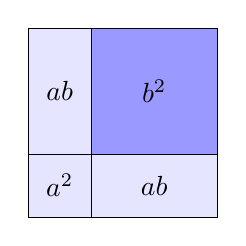
\begin{tikzpicture}[scale=0.8]
\filldraw[fill=blue!10] (0,0) -- (0,1) -- (1,1) -- (1,0) --cycle; % a^2
\draw (0.5,0.5) node{$a^2$};
\filldraw[fill=blue!40] (1,1) -- (1,3) -- (3,3) -- (3,1) --cycle; % b^2
\draw (2,2) node{$b^2$};
\filldraw[fill=blue!10] (1,0) -- (3,0) -- (3,1) -- (1,1) --cycle;
\draw (2,0.5) node{$ab$};
\filldraw[fill=blue!10] (0,1) -- (0,3) -- (1,3) -- (1,1) --cycle;
\draw (0.5,2) node{$ab$};
\end{tikzpicture}


\subsection*{OPPGAVE: $(a-b)^2=a^2-2ab+b^2$}
\subsection*{LØSNING:}
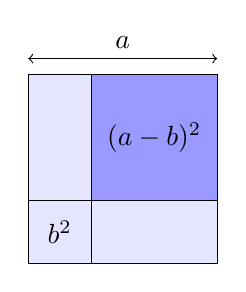
\begin{tikzpicture}[scale=0.8]
\filldraw[fill=blue!10] (0,0) -- (0,1) -- (1,1) -- (1,0) --cycle; % a^2
\draw (0.5,0.5) node{$b^2$};
\filldraw[fill=blue!40] (1,1) -- (1,3) -- (3,3) -- (3,1) --cycle; % b^2
\draw (2,2) node{$(a-b)^2$};
\filldraw[fill=blue!10] (1,0) -- (3,0) -- (3,1) -- (1,1) --cycle;
\filldraw[fill=blue!10] (0,1) -- (0,3) -- (1,3) -- (1,1) --cycle;
\draw[<->] (0,3.25) -- (1.5,3.25) node[anchor=south]{$a$} -- (3,3.25);
\end{tikzpicture}
$=$
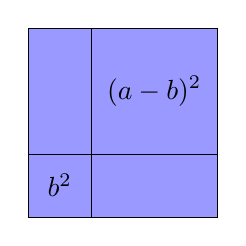
\begin{tikzpicture}[scale=0.8]
\filldraw[fill=blue!40] (0,0) -- (0,1) -- (1,1) -- (1,0) --cycle; % a^2
\draw (0.5,0.5) node{$b^2$};
\filldraw[fill=blue!40] (1,1) -- (1,3) -- (3,3) -- (3,1) --cycle; % b^2
\draw (2,2) node{$(a-b)^2$};
\filldraw[fill=blue!40] (1,0) -- (3,0) -- (3,1) -- (1,1) --cycle;
\filldraw[fill=blue!40] (0,1) -- (0,3) -- (1,3) -- (1,1) --cycle;
\end{tikzpicture}
$-$
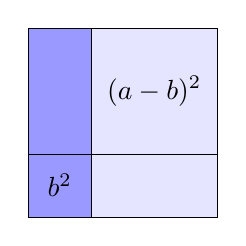
\begin{tikzpicture}[scale=0.8]
\filldraw[fill=blue!40] (0,0) -- (0,1) -- (1,1) -- (1,0) --cycle; %
\draw (0.5,0.5) node{$b^2$};
\filldraw[fill=blue!10] (1,1) -- (1,3) -- (3,3) -- (3,1) --cycle; % 
\draw (2,2) node{$(a-b)^2$};
\filldraw[fill=blue!10] (1,0) -- (3,0) -- (3,1) -- (1,1) --cycle;
\filldraw[fill=blue!40] (0,1) -- (0,3) -- (1,3) -- (1,1) --cycle;
\end{tikzpicture}
$-$
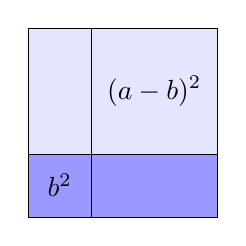
\begin{tikzpicture}[scale=0.8]
\filldraw[fill=blue!40] (0,0) -- (0,1) -- (1,1) -- (1,0) --cycle; %
\draw (0.5,0.5) node{$b^2$};
\filldraw[fill=blue!10] (1,1) -- (1,3) -- (3,3) -- (3,1) --cycle; % 
\draw (2,2) node{$(a-b)^2$};
\filldraw[fill=blue!40] (1,0) -- (3,0) -- (3,1) -- (1,1) --cycle;
\filldraw[fill=blue!10] (0,1) -- (0,3) -- (1,3) -- (1,1) --cycle;
\end{tikzpicture}
$+$
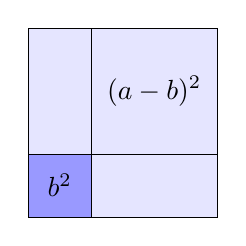
\begin{tikzpicture}[scale=0.8]
\filldraw[fill=blue!40] (0,0) -- (0,1) -- (1,1) -- (1,0) --cycle; % a^2
\draw (0.5,0.5) node{$b^2$};
\filldraw[fill=blue!10] (1,1) -- (1,3) -- (3,3) -- (3,1) --cycle; % b^2
\draw (2,2) node{$(a-b)^2$};
\filldraw[fill=blue!10] (1,0) -- (3,0) -- (3,1) -- (1,1) --cycle;
\filldraw[fill=blue!10] (0,1) -- (0,3) -- (1,3) -- (1,1) --cycle;
\end{tikzpicture}



\subsection*{OPPGAVE: $a^2=b^2+c^2$}
\subsection*{LØSNING:}
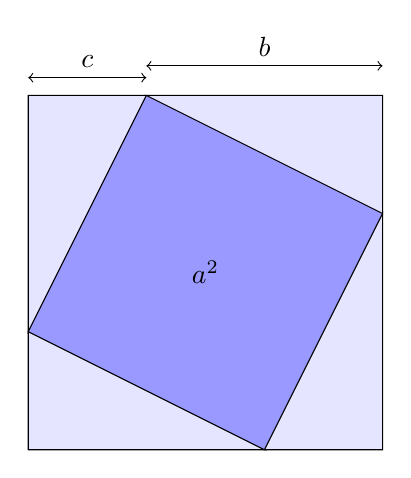
\begin{tikzpicture}[scale=1.5]
\draw[<->] (1,3.25) -- (2,3.25) node[anchor=south]{$b$} -- (3,3.25);
\draw[<->] (0,3.15) -- (.5,3.15) node[anchor=south]{$c$} -- (1,3.15);
\filldraw[fill=blue!40] (0,0) -- (0,3) -- (3,3) -- (3,0) --cycle; %
\filldraw[fill=blue!10] (0,0) -- (0,1) -- (2,0) -- cycle; %
\filldraw[fill=blue!10] (3,0) -- (3,2) -- (2,0) -- cycle; %
\filldraw[fill=blue!10] (3,2) -- (3,3) -- (1,3) -- cycle; %
\filldraw[fill=blue!10] (1,3) -- (0,3) -- (0,1) -- cycle; %
\draw (1.5,1.5) node{$a^2$};
\end{tikzpicture}
$=$
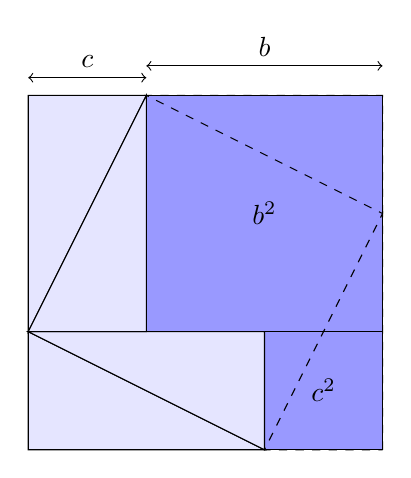
\begin{tikzpicture}[scale=1.5]
\draw[<->] (1,3.25) -- (2,3.25) node[anchor=south]{$b$} -- (3,3.25);
\draw[<->] (0,3.15) -- (.5,3.15) node[anchor=south]{$c$} -- (1,3.15);
\filldraw[fill=blue!40] (0,0) -- (0,3) -- (3,3) -- (3,0) --cycle; %
\filldraw[fill=blue!10] (0,0) -- (0,1) -- (2,0) -- cycle; %
\filldraw[fill=blue!10] (0,1) -- (2,0) -- (2,1) -- cycle; %
\draw[dashed] (3,0) -- (3,2) -- (2,0) -- cycle; %
\draw[dashed] (3,2) -- (3,3) -- (1,3) -- cycle; %
\filldraw[fill=blue!10] (1,3) -- (0,3) -- (0,1) -- cycle; %
\filldraw[fill=blue!10] (0,1) -- (1,1) -- (1,3) -- cycle; %
\draw[] (2,1) -- (3,1); %
\draw (2,2) node{$b^2$};
\draw (2.5,0.5) node{$c^2$};
\end{tikzpicture}

\subsection*{OPPGAVE: $\frac{1}{2}+\frac{1}{2^2}+\frac{1}{2^3}+\frac{1}{2^4}+...+\frac{1}{2^n}+...=1$}
\subsection*{LØSNING:}
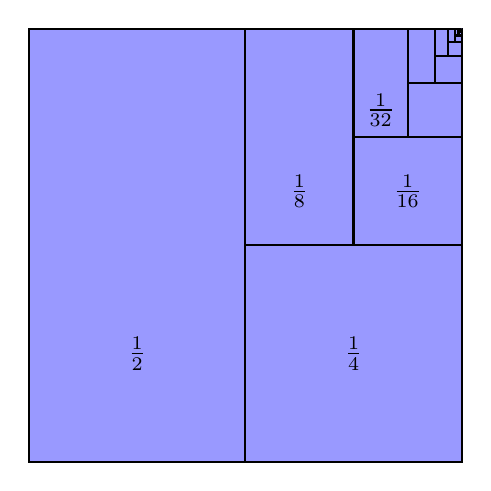
\begin{tikzpicture}[scale=5.5]
\filldraw[fill=blue!0] (0,0) -- (1,0) -- (1,1) -- (0,1) -- cycle; %
\foreach \i in {0,...,25}
{
	\filldraw[thick,fill=blue!40] (1-0.5^\i,1) -- (1-0.5^\i,1-0.5^\i) -- (1-0.5*0.5^\i,1-0.5^\i) -- (1-0.5*0.5^\i,1)-- cycle; %
	\filldraw[thick,fill=blue!40] (1,1-0.5^\i) -- (1,1-0.5*0.5^\i) -- (1-0.5*0.5^\i,1-0.5*0.5^\i) -- (1-0.5*0.5^\i,1-0.5^\i)-- cycle; %
}
\draw (1-2*0.75*0.5^1,1-2*0.75*0.5^1) node{$\frac{1}{2}$};
\draw (1-2*0.75*0.5^2,1-2*0.75*0.5^2) node{$\frac{1}{8}$};
\draw (1-2*0.75*0.5^3,1-2*0.75*0.5^3) node{$\frac{1}{32}$};
\draw (1-2*0.25*0.5^1,1-2*0.75*0.5^1) node{$\frac{1}{4}$};
\draw (1-2*0.25*0.5^2,1-2*0.75*0.5^2) node{$\frac{1}{16}$};
\end{tikzpicture}

\subsection*{OPPGAVE: $a^2+b^2\geq 2ab$}
\subsection*{LØSNING:}
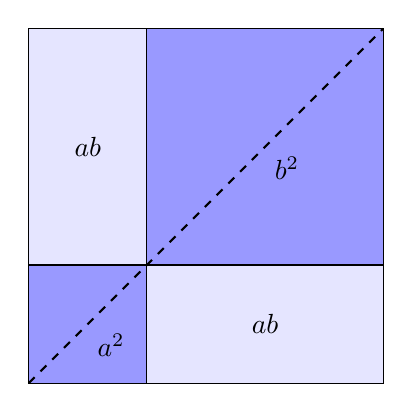
\begin{tikzpicture}[scale=1.5]
\filldraw[fill=blue!40] (0,0) -- (0,1) -- (1,1) -- (1,0) --cycle; % a^2
\draw (0.5,0.5) node[anchor=north west]{$a^2$};
\filldraw[fill=blue!40] (1,1) -- (1,3) -- (3,3) -- (3,1) --cycle; % b^2
\draw (2,2) node[anchor=north west]{$b^2$};
\filldraw[fill=blue!10] (1,0) -- (3,0) -- (3,1) -- (1,1) --cycle;
\draw (2,0.5) node{$ab$};
\filldraw[fill=blue!10] (0,1) -- (0,3) -- (1,3) -- (1,1) --cycle;
\draw (0.5,2) node{$ab$};
\draw[thick,dashed] (0,0) -- (3,3);
\end{tikzpicture}
$\rightarrow$
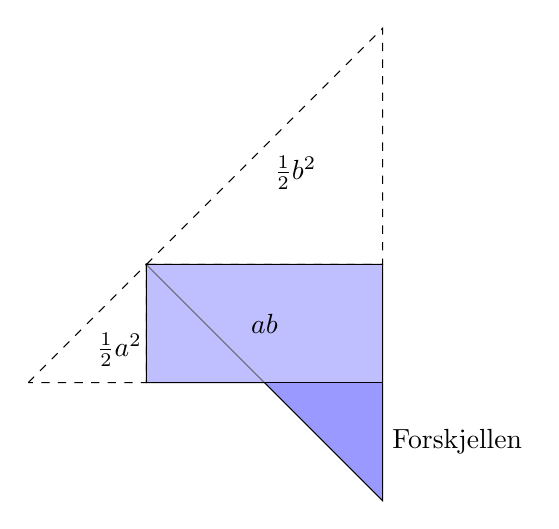
\begin{tikzpicture}[scale=1.5]
\filldraw[dashed,fill=blue!0] (0,0) -- (1,1) -- (1,0) --cycle; % a^2
\filldraw[dashed,fill=blue!0] (1,1) -- (3,3) -- (3,1) --cycle; % b^2
\filldraw[fill=blue!40] (2,0) -- (1,1) -- (1,0) --cycle; % a^2
\filldraw[fill=blue!40] (1,1) -- (3,-1) -- (3,1) --cycle; % b^2
\filldraw[fill=blue!10,fill opacity=0.5] (1,0) -- (3,0) -- (3,1) -- (1,1) --cycle;
\draw (2,0.5) node{$ab$};
\draw (2,2) node[anchor=north west]{$\frac{1}{2}b^2$};
\draw (0.5,0.5) node[anchor=north west]{$\frac{1}{2}a^2$};
\draw (3,-0.5) node[anchor=west]{Forskjellen};
\end{tikzpicture}


\subsection*{OPPGAVE: $1+2+3+4+...+(N-1)+N=\frac{1}{2}N(N+1)$}
\subsection*{LØSNING:}
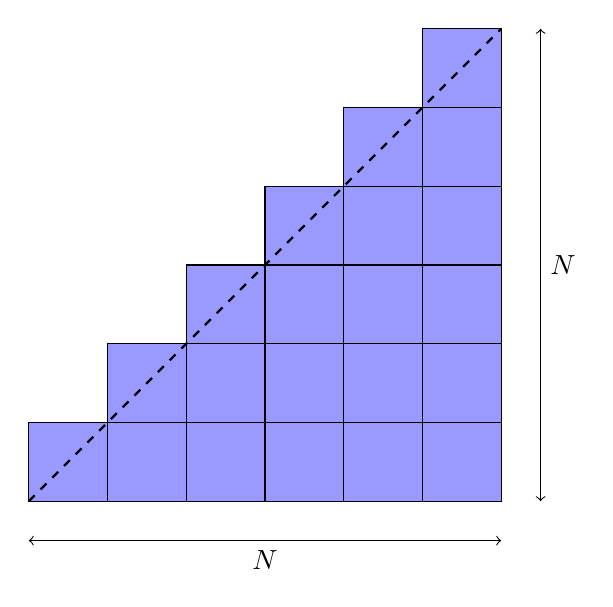
\begin{tikzpicture}
\foreach \i in {1,...,6}
{
	\filldraw[fill=blue!40] (\i-1,0) -- (\i,0) -- (\i,\i) -- (\i-1,\i) -- cycle;	
}
\foreach \i in {1,...,6}
{
	\draw (\i-1,\i-1) -- (6,\i-1);
}
\draw[thick,dashed] (0,0) --(6,6);
\draw[<->] (0,-.5) -- (3,-.5) node[anchor=north]{$N$} -- (6,-.5);
\draw[<->] (6.5,0) -- (6.5,3) node[anchor=west]{$N$} -- (6.5,6);
\end{tikzpicture}
$=\frac{1}{2}N^2+\frac{1}{2}N=\frac{1}{2}N(N+1)$

\subsection*{}
\subsection*{}
\subsection*{}
\subsection*{}
\subsection*{}
  
  
\end{document}












